\documentclass[a4paper]{article}

%% Language and font encodings
\usepackage[english]{babel}
\usepackage[utf8x]{inputenc}
\usepackage[T1]{fontenc}
\usepackage[]{enumitem}
\usepackage[table]{xcolor}
\usepackage{amsmath}



%% Sets page size and margins
\usepackage[a4paper,top=3cm,bottom=2cm,left=3cm,right=3cm,marginparwidth=1.75cm]{geometry}

%% Useful packages
\usepackage{amsmath}
\usepackage{graphicx}
\usepackage[colorinlistoftodos]{todonotes}
\usepackage[colorlinks=true, allcolors=blue]{hyperref}

\title{
  Week 1 Check-in\\
  \large EAE 3600 - 3D Modeling}
\author{Jesus Zarate}

\begin{document}
\maketitle

\begin{figure}[h]
\centering
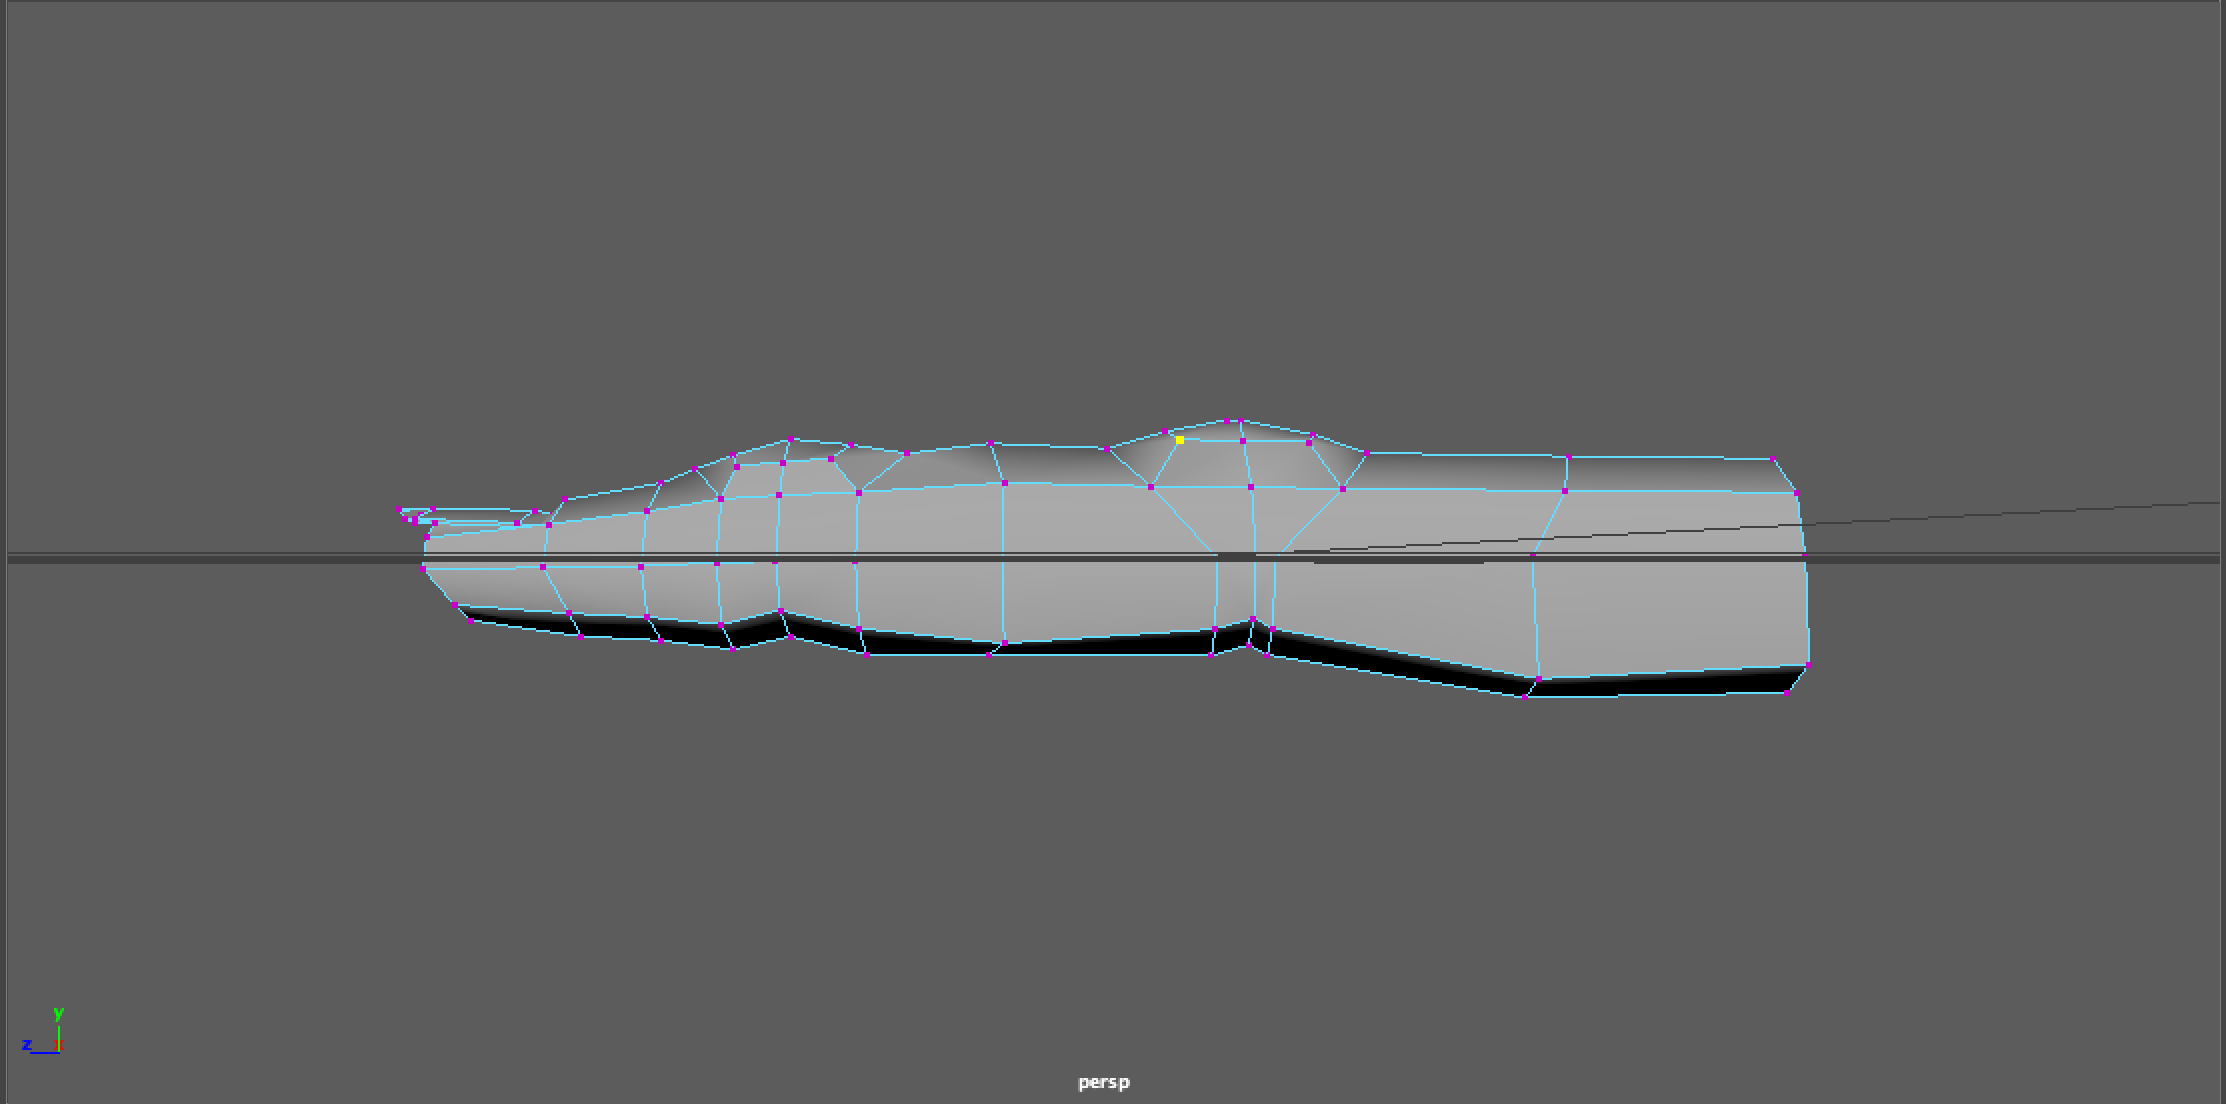
\includegraphics[width=10cm]{img/SideView.png}
\caption{Side View.}
\label{fig:Side View}
\end{figure}

\begin{figure}[h]
\centering
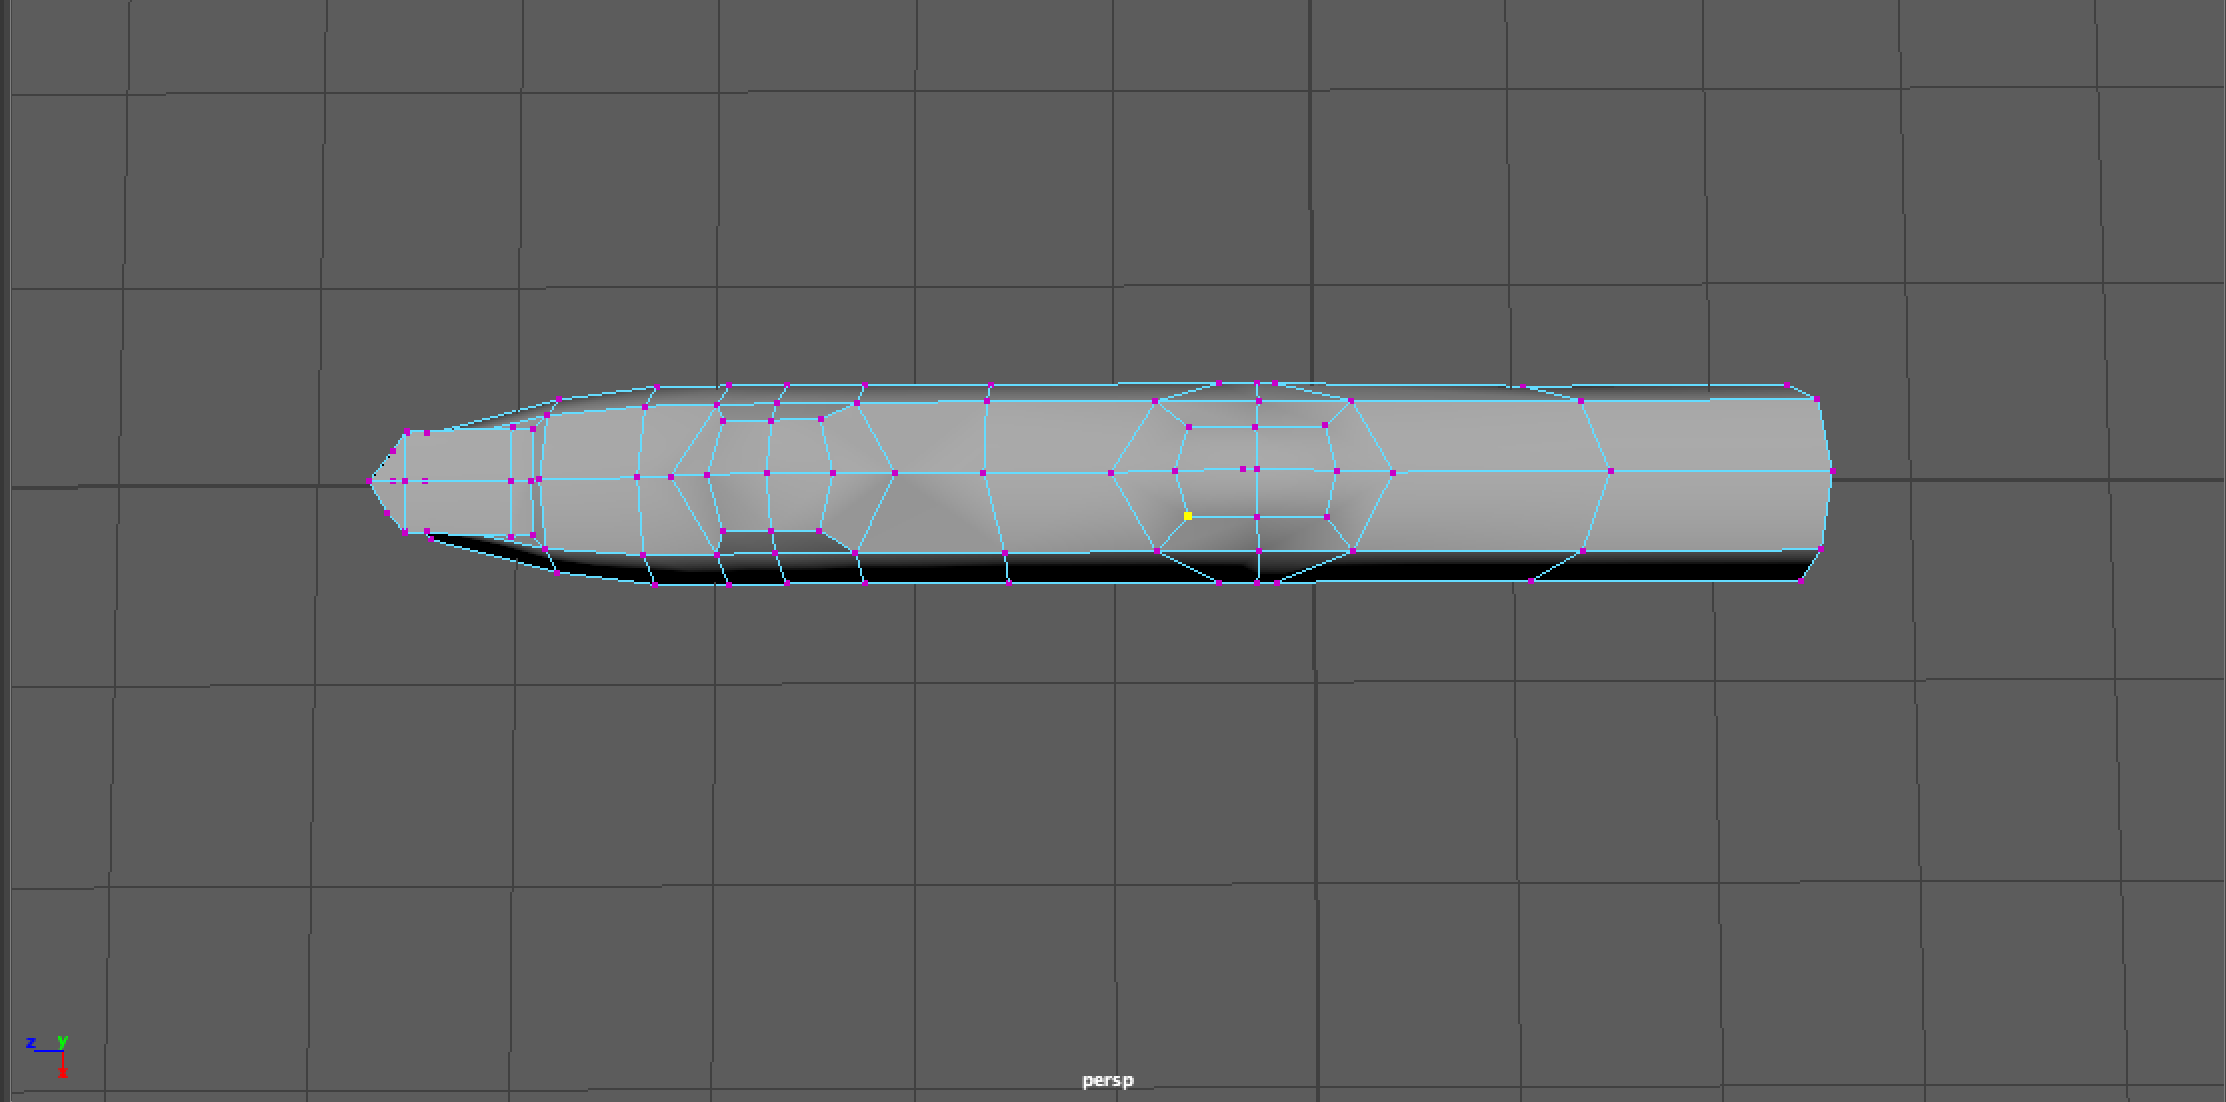
\includegraphics[width=10cm]{img/TopView.png}
\caption{Top View.}
\label{fig:Top View}
\end{figure}

\begin{figure}[h]
\centering
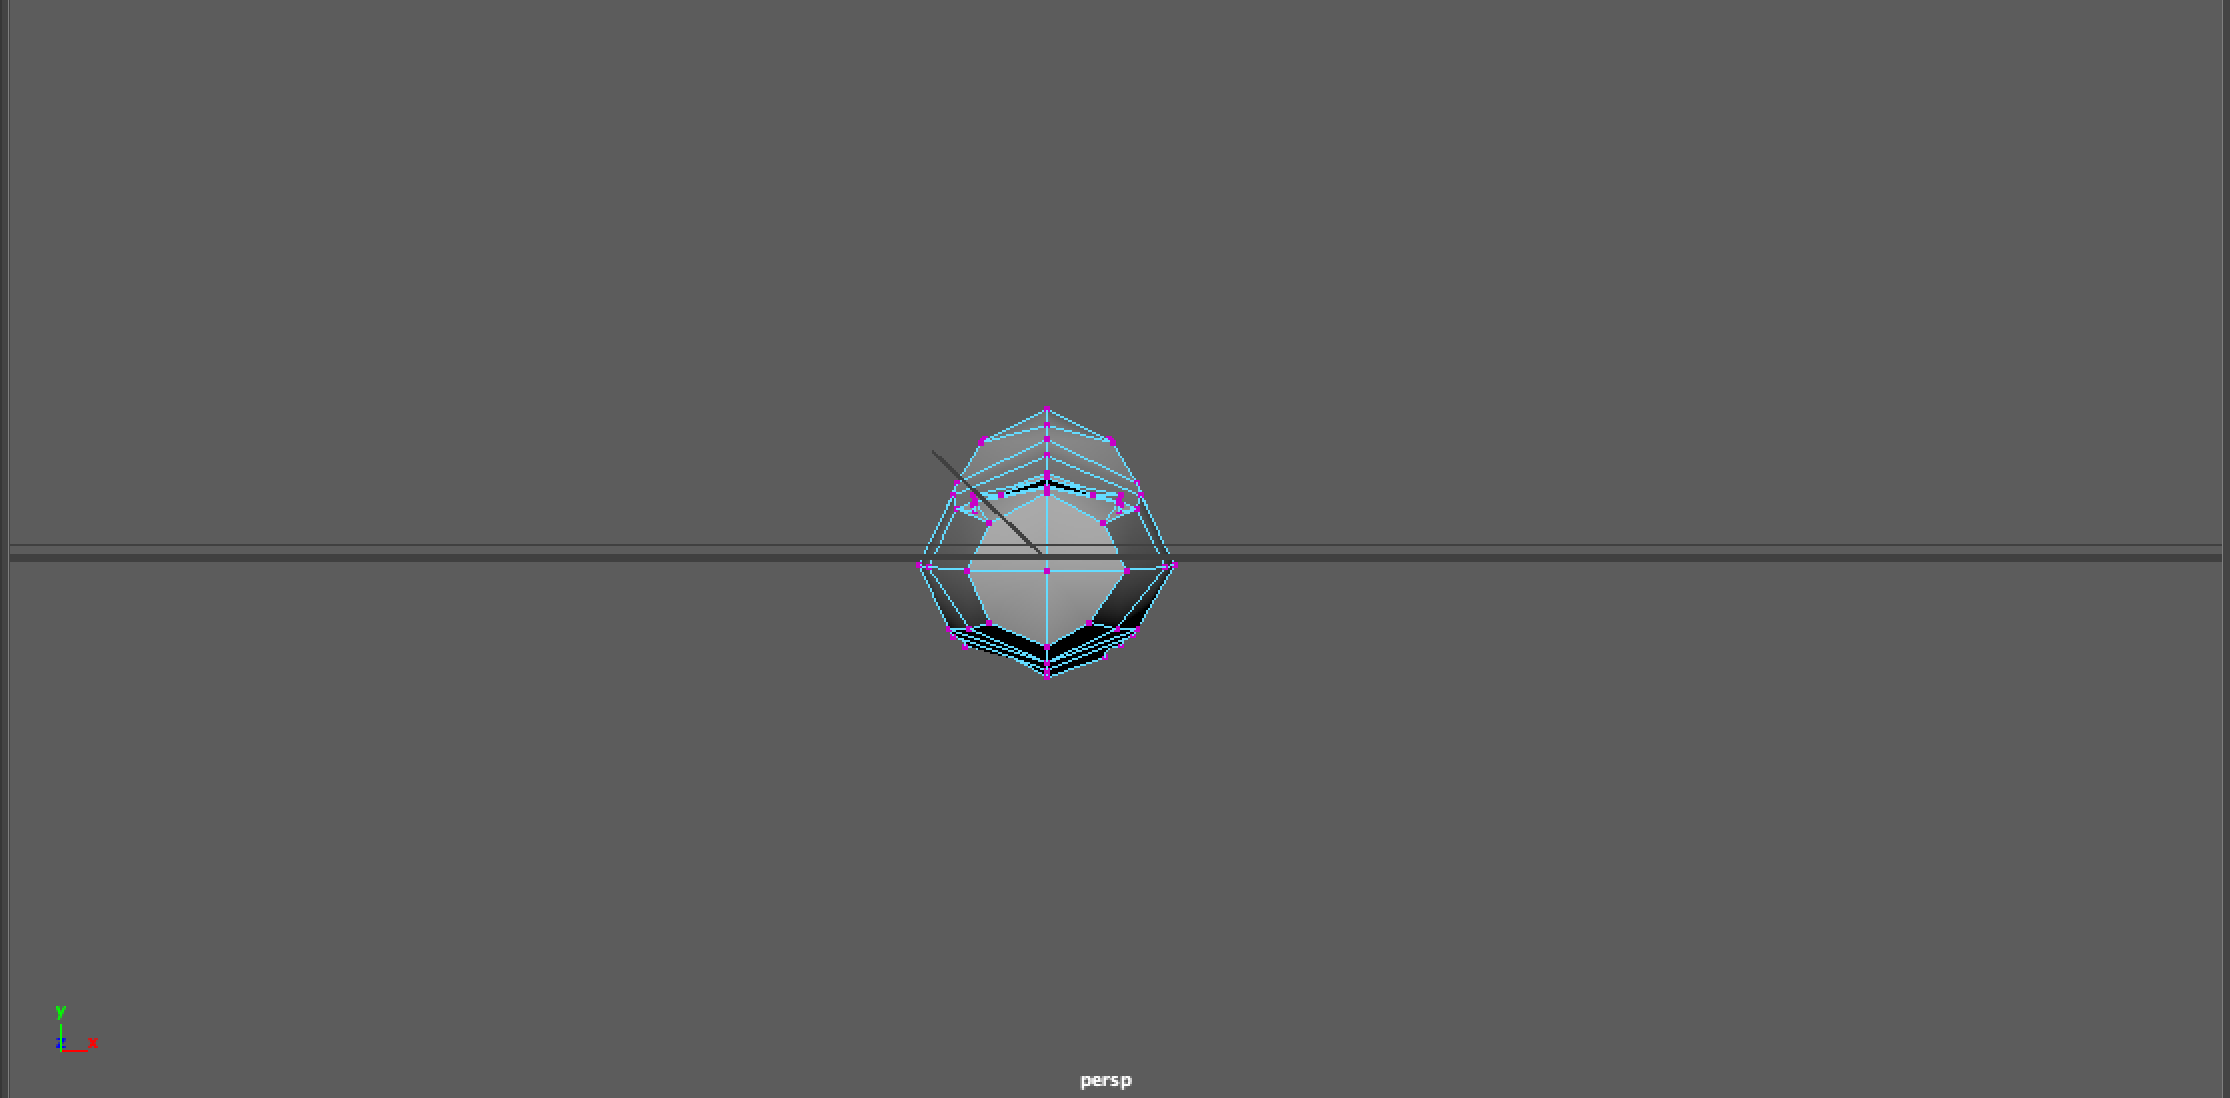
\includegraphics[width=10cm]{img/FrontView.png}
\caption{Front View}
\label{fig:Front View}
\end{figure}

\begin{figure}[h]
\centering
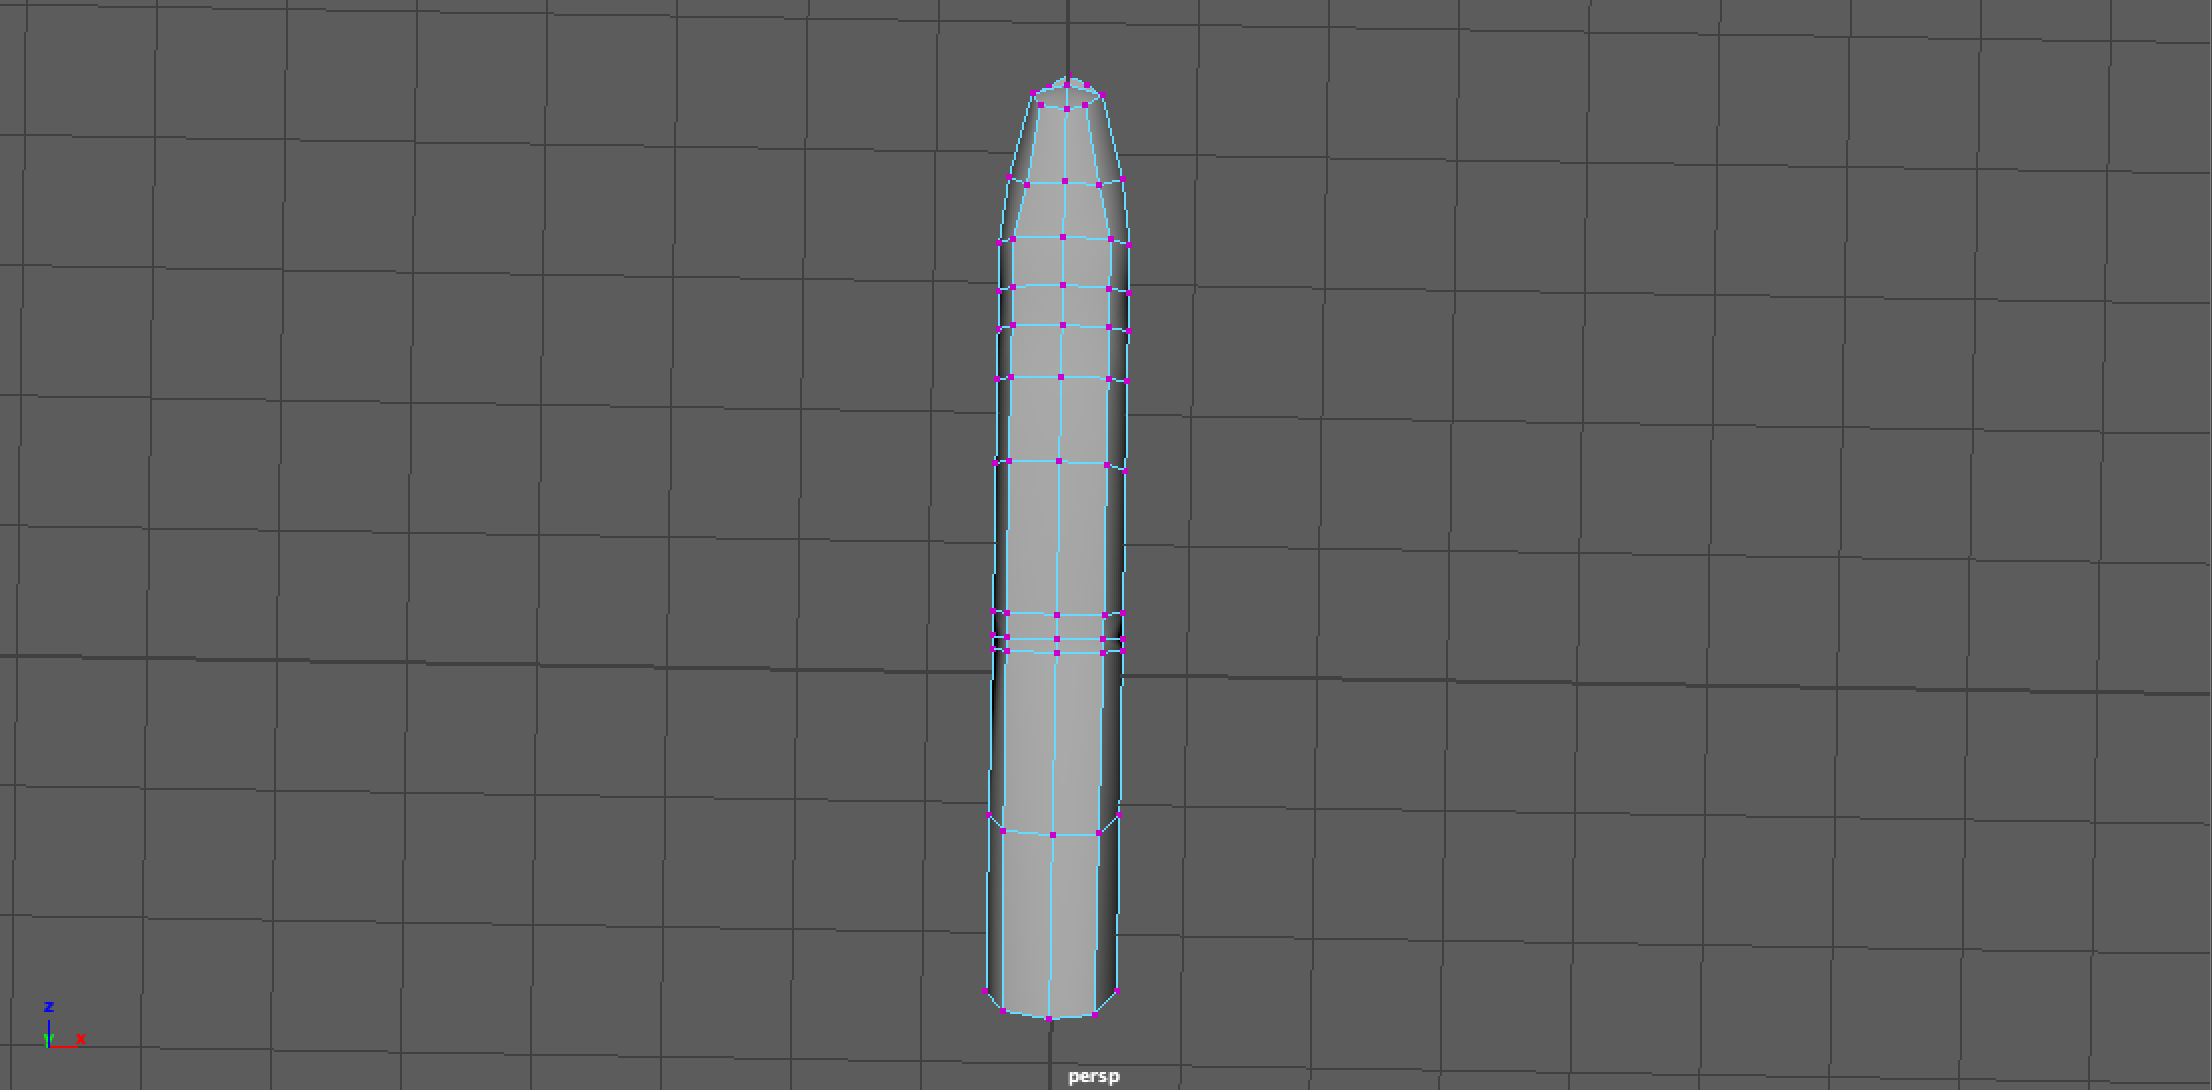
\includegraphics[width=10cm]{img/BottomView.png}
\caption{Bottom View}
\label{fig:Bottom View}
\end{figure}

\begin{figure}[h]
\centering

\includegraphics[width=10cm]{img/GENJI.jpg}
\caption{Genji}
\label{fig:Gengi}
\end{figure}


\end{document}
